\documentclass{article}

\usepackage{amsmath}
\usepackage{fancyhdr}
\usepackage{graphicx}
\graphicspath{{}}

%% some colours
\usepackage{color}
\definecolor{deepblue}{rgb}{0,0,0.5}
\definecolor{deepred}{rgb}{0.6,0,0}
\definecolor{deepgreen}{rgb}{0,0.5,0}
\definecolor{backcolour}{rgb}{0.95,0.96,0.93}

%%%%%%%%%%%%%% CODE STUFF %%%%%%%%%%%%%%
%%%%%%%%%%%%%%%%%%%%%%%%%%%%%%%%%%%%%%%%
\usepackage{cprotect} % to be used in sol
\usepackage{listings} % for code display
% setting code style
\newcommand\pythonstyle{\lstset{
        language=Python,
        backgroundcolor=\color{backcolour},
		basicstyle=\footnotesize,
		otherkeywords={self},
		keywordstyle=\footnotesize\color{deepblue},
		emph={__init__},
		emphstyle=\footnotesize\color{deepred},
		stringstyle=\color{deepgreen},
		frame=single,
		showstringspaces=false  ,
		breaklines=true,
		numbers=left,
		numberstyle=\footnotesize,
		tabsize=4,
		breakatwhitespace=false
	}}

% Python environment
\lstnewenvironment{python}[1][]{
    \pythonstyle
    \lstset{#1}
}{}

% Python for external files
\newcommand\pythonexternal[2][]{{
    \pythonstyle
    \lstinputlisting[#1]{#2}
}}

% Python for inline
\newcommand\pythoninline[1]{{\pythonstyle\lstinline!#1!}}

%%%%%%%%%%%%%%%%%%%%%%%%%%%%%%%%%%%%%%%%
% setting the style for ex documents
\pagestyle{fancy}
\fancyhf{}
\fancyhead[L]{\thetitle}
\fancyhead[C]{}
\fancyhead[R]{\theauthor}
\renewcommand{\headrulewidth}{0.4pt} %obere Trennlinie
\fancyfoot[L]{Due: \thedate}
\fancyfoot[R]{\thepage} %Seitennummer
\renewcommand{\footrulewidth}{0.4pt}

% include solutions
\newcommand\sol[1]{{\large\textbf{\\Solution:}}#1}
\usepackage{tikz}
\usetikzlibrary{arrows,automata}

\title{BPP Exercise 6 - Sorting and IO}
\author{A. Hain, M. Nipshagen}
\date{14.05.2018, 08:00}

\makeatletter
\let\thetitle\@title
\let\theauthor\@author
\let\thedate\@date
\makeatother

% do not include solutions
% \renewcommand\sol[1]{}


\begin{document}

The deadline for this exercise sheet is \textbf{Monday, \thedate.}
%
%\section*{Introductory Words}
%In case we have some information that doesn't directly concern the current exercises.
%

\section{Warm-Up}

\subsection{Key Sort}
Given a list of the following structure:
\begin{python}
my_lst = [
  {
    "key1" : value1,
    "key2" : value2,
    "key3" : value3
  },
  {
    "key1" : a_value,
    "key2" : b_value,
    "key3" : c_value
  },
  ...
]
\end{python}
Sort the list in such a way, that the value of \texttt{"key2"} is used to compare and sort the dictionaries inside the list. In the file 
\texttt{task\_1.py} you can find an example dictionary as well as a sorted
version to compare to when you are done.
\\
\cprotect\sol{
\begin{python}
sorted(my_lst, key=lambda x: x["key2"])
\end{python}
}

\subsection{Read \& Write}
In the file \texttt{task\_1.txt}, is an unsorted list of numbers. Read in the list, sort it in \textit{descending} order and write it back to the file.
In the end the file should only contain the sorted list.\\
\cprotect\sol{
\begin{python}
import re


with open("./task_1.txt", "r+") as f:
    lst_in = f.read() # read the list as string
    lst_in = re.sub("(\[|\])", "", lst_in) # get rid of the brackets
    # split on the commas of the list,
    # and cast to float since we are dealing with numbers
    lst = [float(x) for x in lst_in.split(",")]
    lst.sort(reverse=True) # and sort
    f.write(str(lst)) # back in the file it goes
\end{python}
}

\section{Powering through I/O}
Let's make a game! In Hangman, one player -- in our case this will be the
computer -- picks a random word and tells the other player(s) how many
letters it has -- usually displayed through underscores. For example, if
the word is \texttt{hello} we would get \verb|_ _ _ _ _|.\\
The other player(s) now have to guess the word letter by letter. If a
letter that is part of the word is guessed, it is revealed. To
continue our example, if you would guess an \textbf{e} the computer would
reveal it and the new game state would be \verb|_ e _ _ _|. If your next
guess would be an \textbf{l} the new game state would be \verb|_ e l l _|.
If you guessed the whole word, you win the game!\\
But there is a catch: Traditionally, at the start of the game you would
draw empty gallows, and every time you guessed a letter that is
\textit{not} in the word, you would draw one more part of a man hanging --
thus the name hangman (see \ref{fig:hangman}). If you guess the word
before the man is complete, you win! Otherwise the stick figure has 
come to a tragic end and you lose.\\
Since it might be hard to visualise the hangman on the terminal (you are 
very welcome to try it out though), you might want to use just a counter.

\subsection*{Task}
Write a \texttt{hangman.py} script which implements a version of the 
hangman game. In the supplied \textbf{.zip} file you can find a 
\texttt{words.txt}, which you should use to read in the list of possible
words. You are welcome to change the file though.\\
An example pseudocode:
\begin{verbatim}
Set number of misses
Read in possible words
Choose a word
Prepare guessword with underscores
Display the rule set
While not guessed and more than 0 misses left:
  Display current game state
  Get a guess letter as user input
  If guessed letter is in the word:
    Update the guess word
    If guessed:
      win
  Else:
    Update list of failes and misses
    If no misses left:
      Lose
\end{verbatim}

\subsection*{Hints}
\begin{itemize}
  \item Remember that strings are immutable, so you can not do:
\begin{python}
a = 'hello'
a[3] = 'a
\end{python}
  \item You can instead display the guessword as a list of underscores
\begin{python}
word = 'hello'
guess_word = ['_', '_', '_', '_', '_']
\end{python}
  \item Whenever you have gotten an input letter, check whether it is
  part of the word. You can use the \pythoninline{in} keyword and the
  \pythoninline{word.index(input_char)} function for this.
\begin{python}
if 'l' in word:
  guess_word[word.index('l')] = 'l'
\end{python}
\emph{Note:} This code snippet probably is not how you are going to
use it. But it might point you in the right direction.
  \item Similarly, you can use \texttt{in} to check whether the player
  has won.
  \item For choosing a word, you could take a look at the \texttt{choice}
  function from the \texttt{random} module. You can read upon it here:
  \url{https://docs.python.org/3.5/library/random.html#random.choice}.\\
  And you can use it with the following structure:
\begin{python}
import random


random.choise(my_list)
\end{python}
\end{itemize}
It might be a good idea to split your code into several smaller functions,
which each perform a single task. For example, one function which checks
whether the player has won, one function to print the current game state,
one to read in the file, and one to pick a word, and so on. Then combine
those functions to build your whole game.\\
Please note, that the hints are just that: hints for a possible solution
to a problem. Your program can be perfectly fine without using any of
the hints.


\begin{figure}[h]
\centering
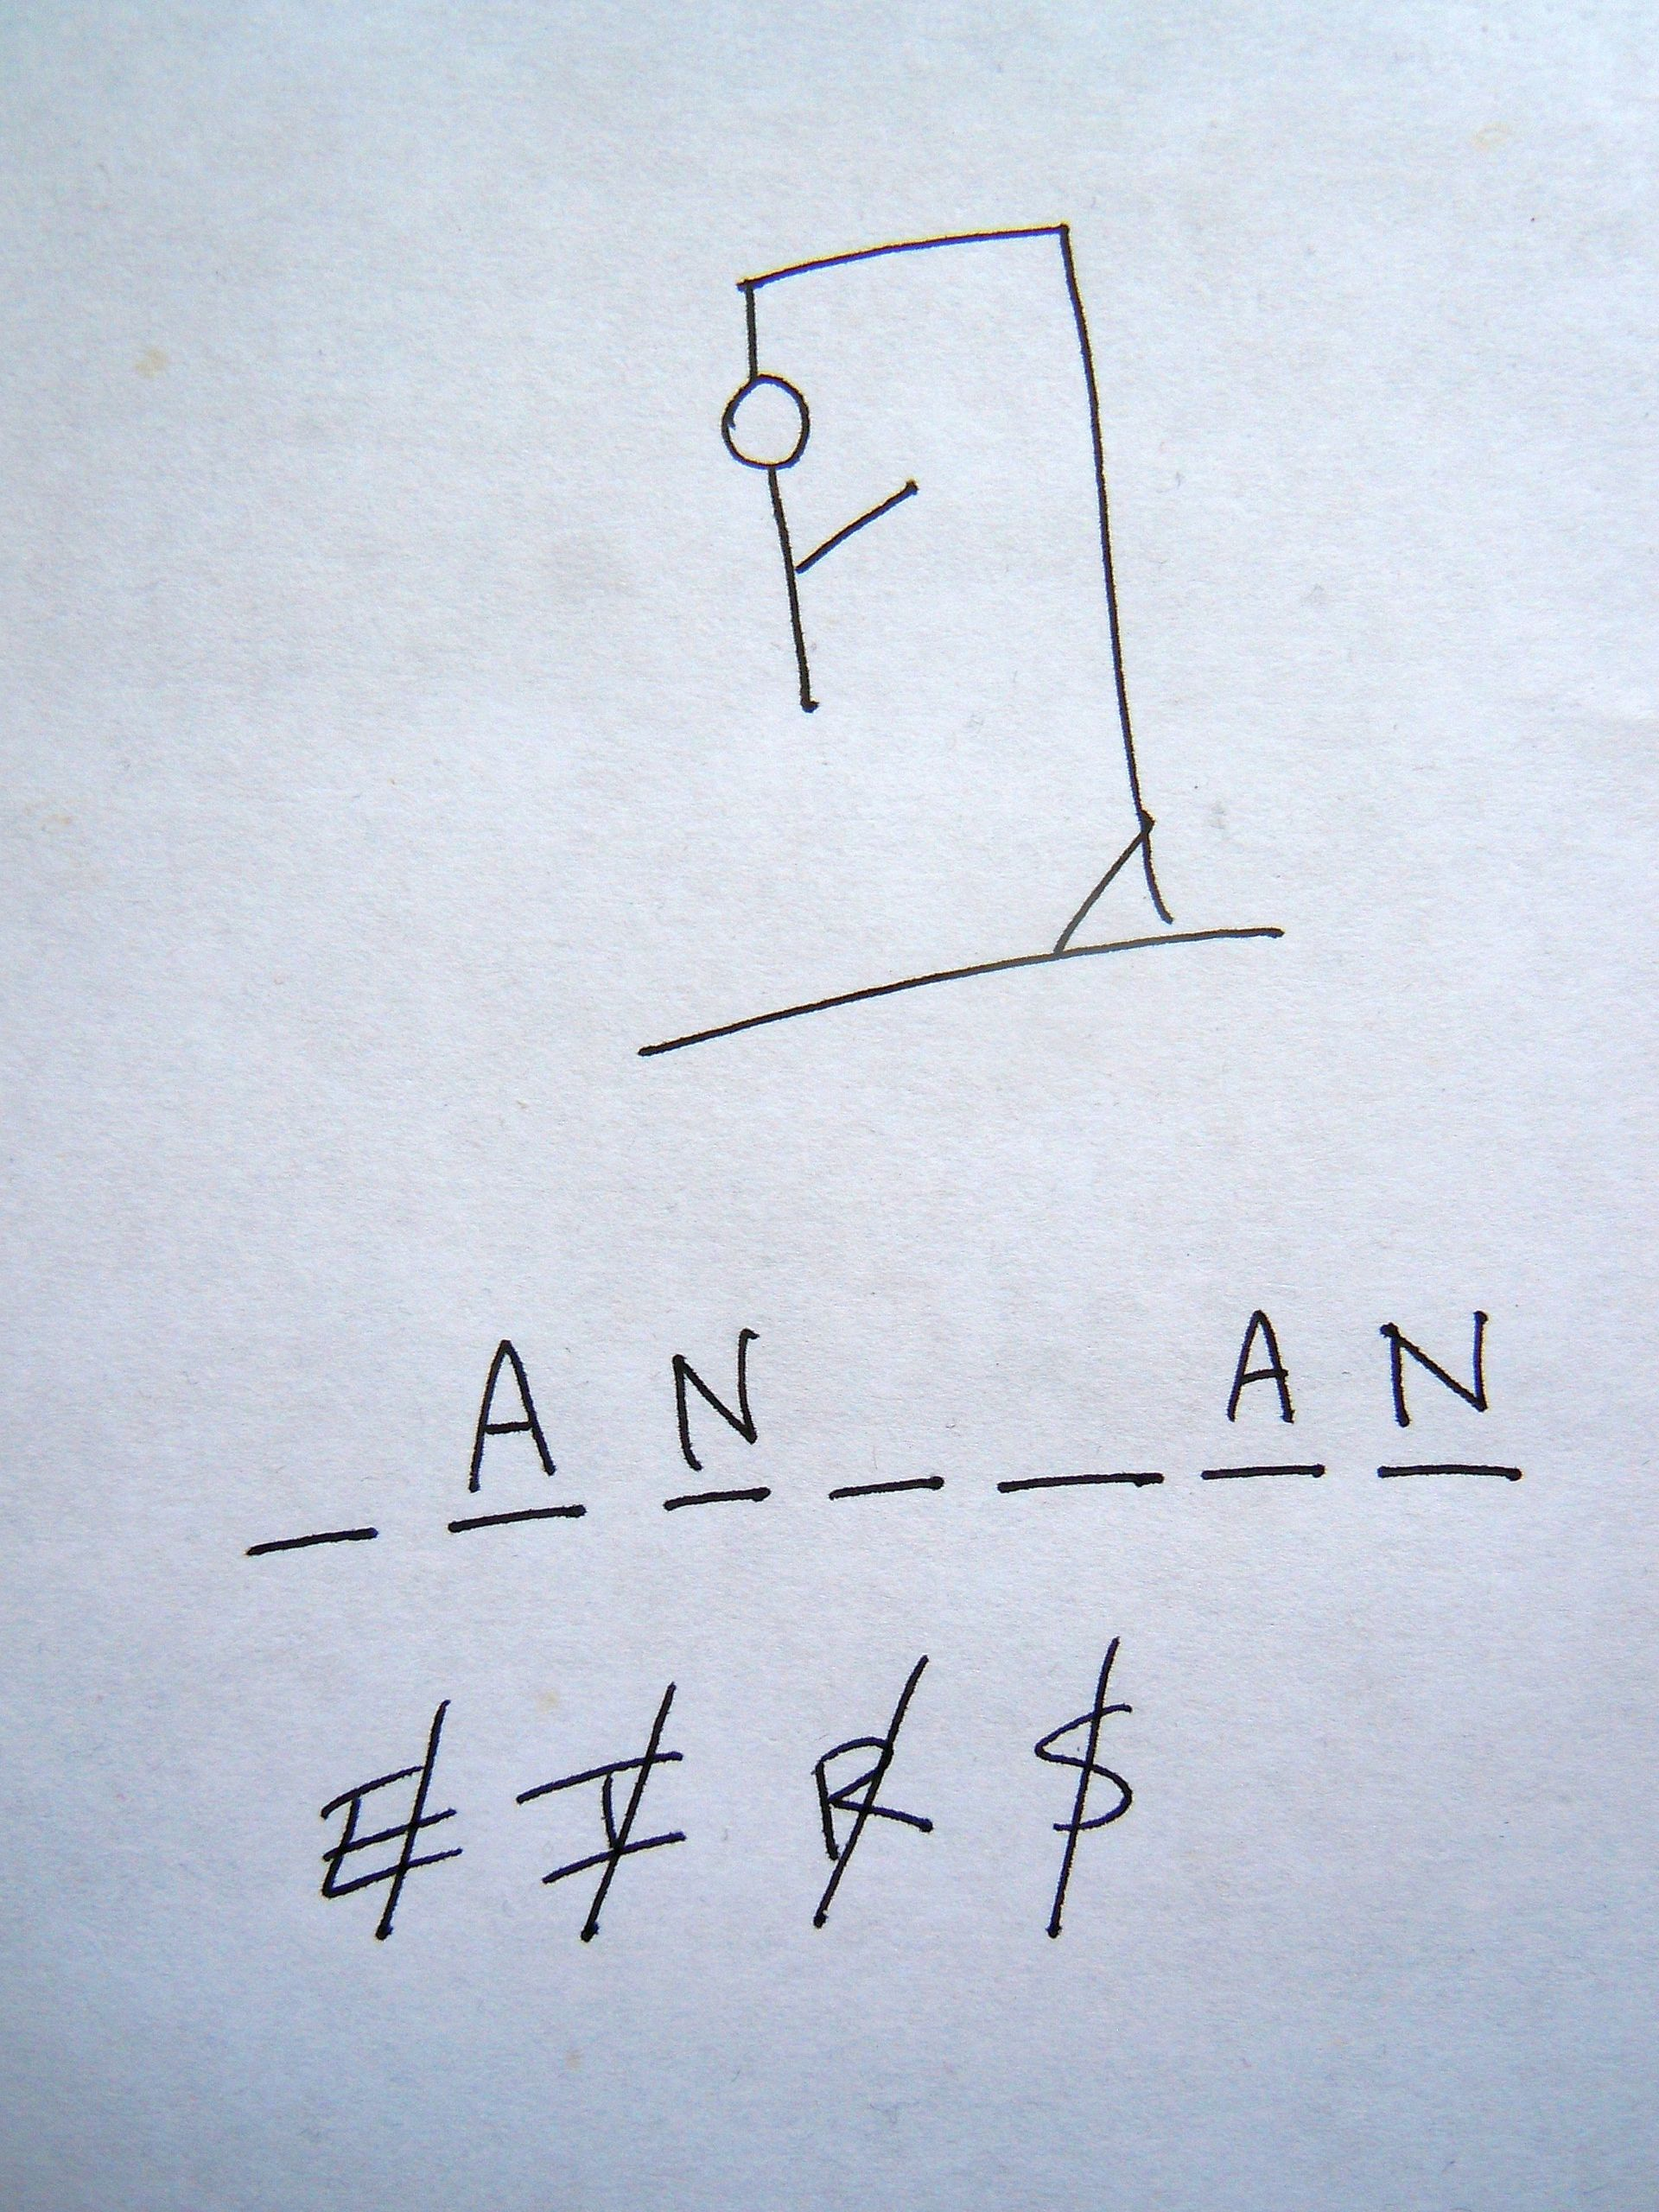
\includegraphics[width=0.8\textwidth]{hangman}
\label{fig:hangman}
\caption{Example hangman game}
\small{Taken from \url{https://upload.wikimedia.org/wikipedia/commons/thumb/f/f4/Hangman_game.jpg/1920px-Hangman_game.jpg}}
\end{figure}

\end{document}
